\documentclass{article}

\usepackage{nips_2018_author_response}

\usepackage[utf8]{inputenc} % allow utf-8 input
\usepackage[T1]{fontenc}    % use 8-bit T1 fonts
\usepackage{hyperref}       % hyperlinks
\usepackage{url}            % simple URL typesetting
\usepackage{booktabs}       % professional-quality tables
\usepackage{amsfonts}       % blackboard math symbols
\usepackage{nicefrac}       % compact symbols for 1/2, etc.
\usepackage{microtype}      % microtypography
\usepackage{xcolor}

\usepackage{wrapfig}
\usepackage{picins}

\usepackage{amsmath}
\usepackage{amssymb}
\usepackage{amsthm}
\usepackage{algorithm}
\usepackage[noend]{algorithmic}
%\usepackage{algpseudocode}
\usepackage{graphicx}

\usepackage{ulem}

\begin{document}

{\bf Reviewer 1: }
1. 
Thanks for the references---mirror descent (MD) is an ubiquitous idea.
We note that [Liu et al., 2015] is not closely related,
given that it considers the much simpler task of policy evaluation,
whereas our focus is on policy optimization.
At a high level,
the [Thomas et al. 2013] paper is more relevant,
but there are fundamental differences:
our focus is on investigating efficient exploration,
whereas [Thomas et al. 2013] focus on learning safe policies.
We also modify the traditional MD framework,
based on a reversal of the KL divergence,
which is a critical step not considered by [Thomas et al. 2013].
More importantly, the alternative approach we develop allows for
performance guarantees in the \emph{non-convex} setting 
(see next comment).

2. There seems to be a basic misunderstanding of the key technical
contribution of this paper:
The main result does not require convexity;
instead, we make the much weaker assumption that the optimization 
problem Eq.(6) is solvable.
Moreover:
(1) Solving {\small $\arg\max_{\pi \in \Pi} \mathbb{E}r(\rho) - \tau D_{\text{KL}}(\pi \| \pi_{\theta_t}) + \tau' \text{H}(\pi)$}. Instead, we firstly solve it in the simplex space, which has an analytical solution, and then perform a projection step. 
(2) Solving the projection step, $\pi_\theta$, is still difficult for a 
general neural network, but it is solvable in some specific non-convex cases. 
Consider the widely used parameterized softmax policies 
{\small $\pi_{\theta} \triangleq 
\exp\left\{\Phi^\top\theta\right\}/
{{\mathbf{1}^\top \exp\left\{\Phi^\top\theta\right\}}}$}, 
where {\small $\Phi\in \mathbb{R}^{K\times A}$} is the feature matrix, 
$A$ is the number of actions, $K$ is the dimension of features, 
and $\theta$ is the policy parameter. 
Note that the policy space is non-convex and $K\ll A$ 
as in Sec 4.1.1. Standard MD cannot exactly solve this projection step 
because $\text{KL}(\pi_{\theta} \| q)$ is non-convex in $\theta$.
On the other hand, our paper proposes to use the reversed entropy
$\text{KL}(q \| \pi_{\theta})$, which is actually convex for $\theta$
(note that {\small $\frac{d^2 \text{KL}(q \| \pi_{\theta})}{d \theta^2} 
= \Phi (\Delta(\pi_\theta) - \pi_\theta \pi_\theta^\top) \Phi^\top \succeq 0$}). 
It is also worth noting that this is similar with the 1-layer NN case.
(For more general NN architectures, 
further understanding of the behavior of the NN is needed.)

3. Although we agree that the two experiments in [Thomas et al., 2013]
are interesting, we do not agree that these necessarily constitute
``a better suite of experiments''.
(We did not consider ``trivial toy video games'',
so that comment must be directed elsewhere.)
There is significant value to having shared domains
with reproducible benchmarks to gauge progress in a community.
Certainly there are risks, 
analogous to the over-use of UCI data in supervised learning,
but there are scientific benefits to being able to compare
results across different labs and approaches.
Simpler benchmarks become supplanted by more challenging ones 
when methods become sufficiently capable, such as ImageNet supplanting MNIST
and Cifar-10, but not before then.
By contrast, no one outside the UMass lab where [Thomas et al. 2013] conducted 
their robot balancing experiment is going to be able to reproduce their
findings.
Using complicated yet non-open-source simulators also hampers reproducibility
and complicates the fundamental understanding of different methods.
Also,
if a shared domain is too challenging
it ceases being immediately useful for evaluating current methods.

\piccaption[]{reward and exp-reward over $\theta$.\label{fig:exp_reward_over_theta}}
\parpic[r]{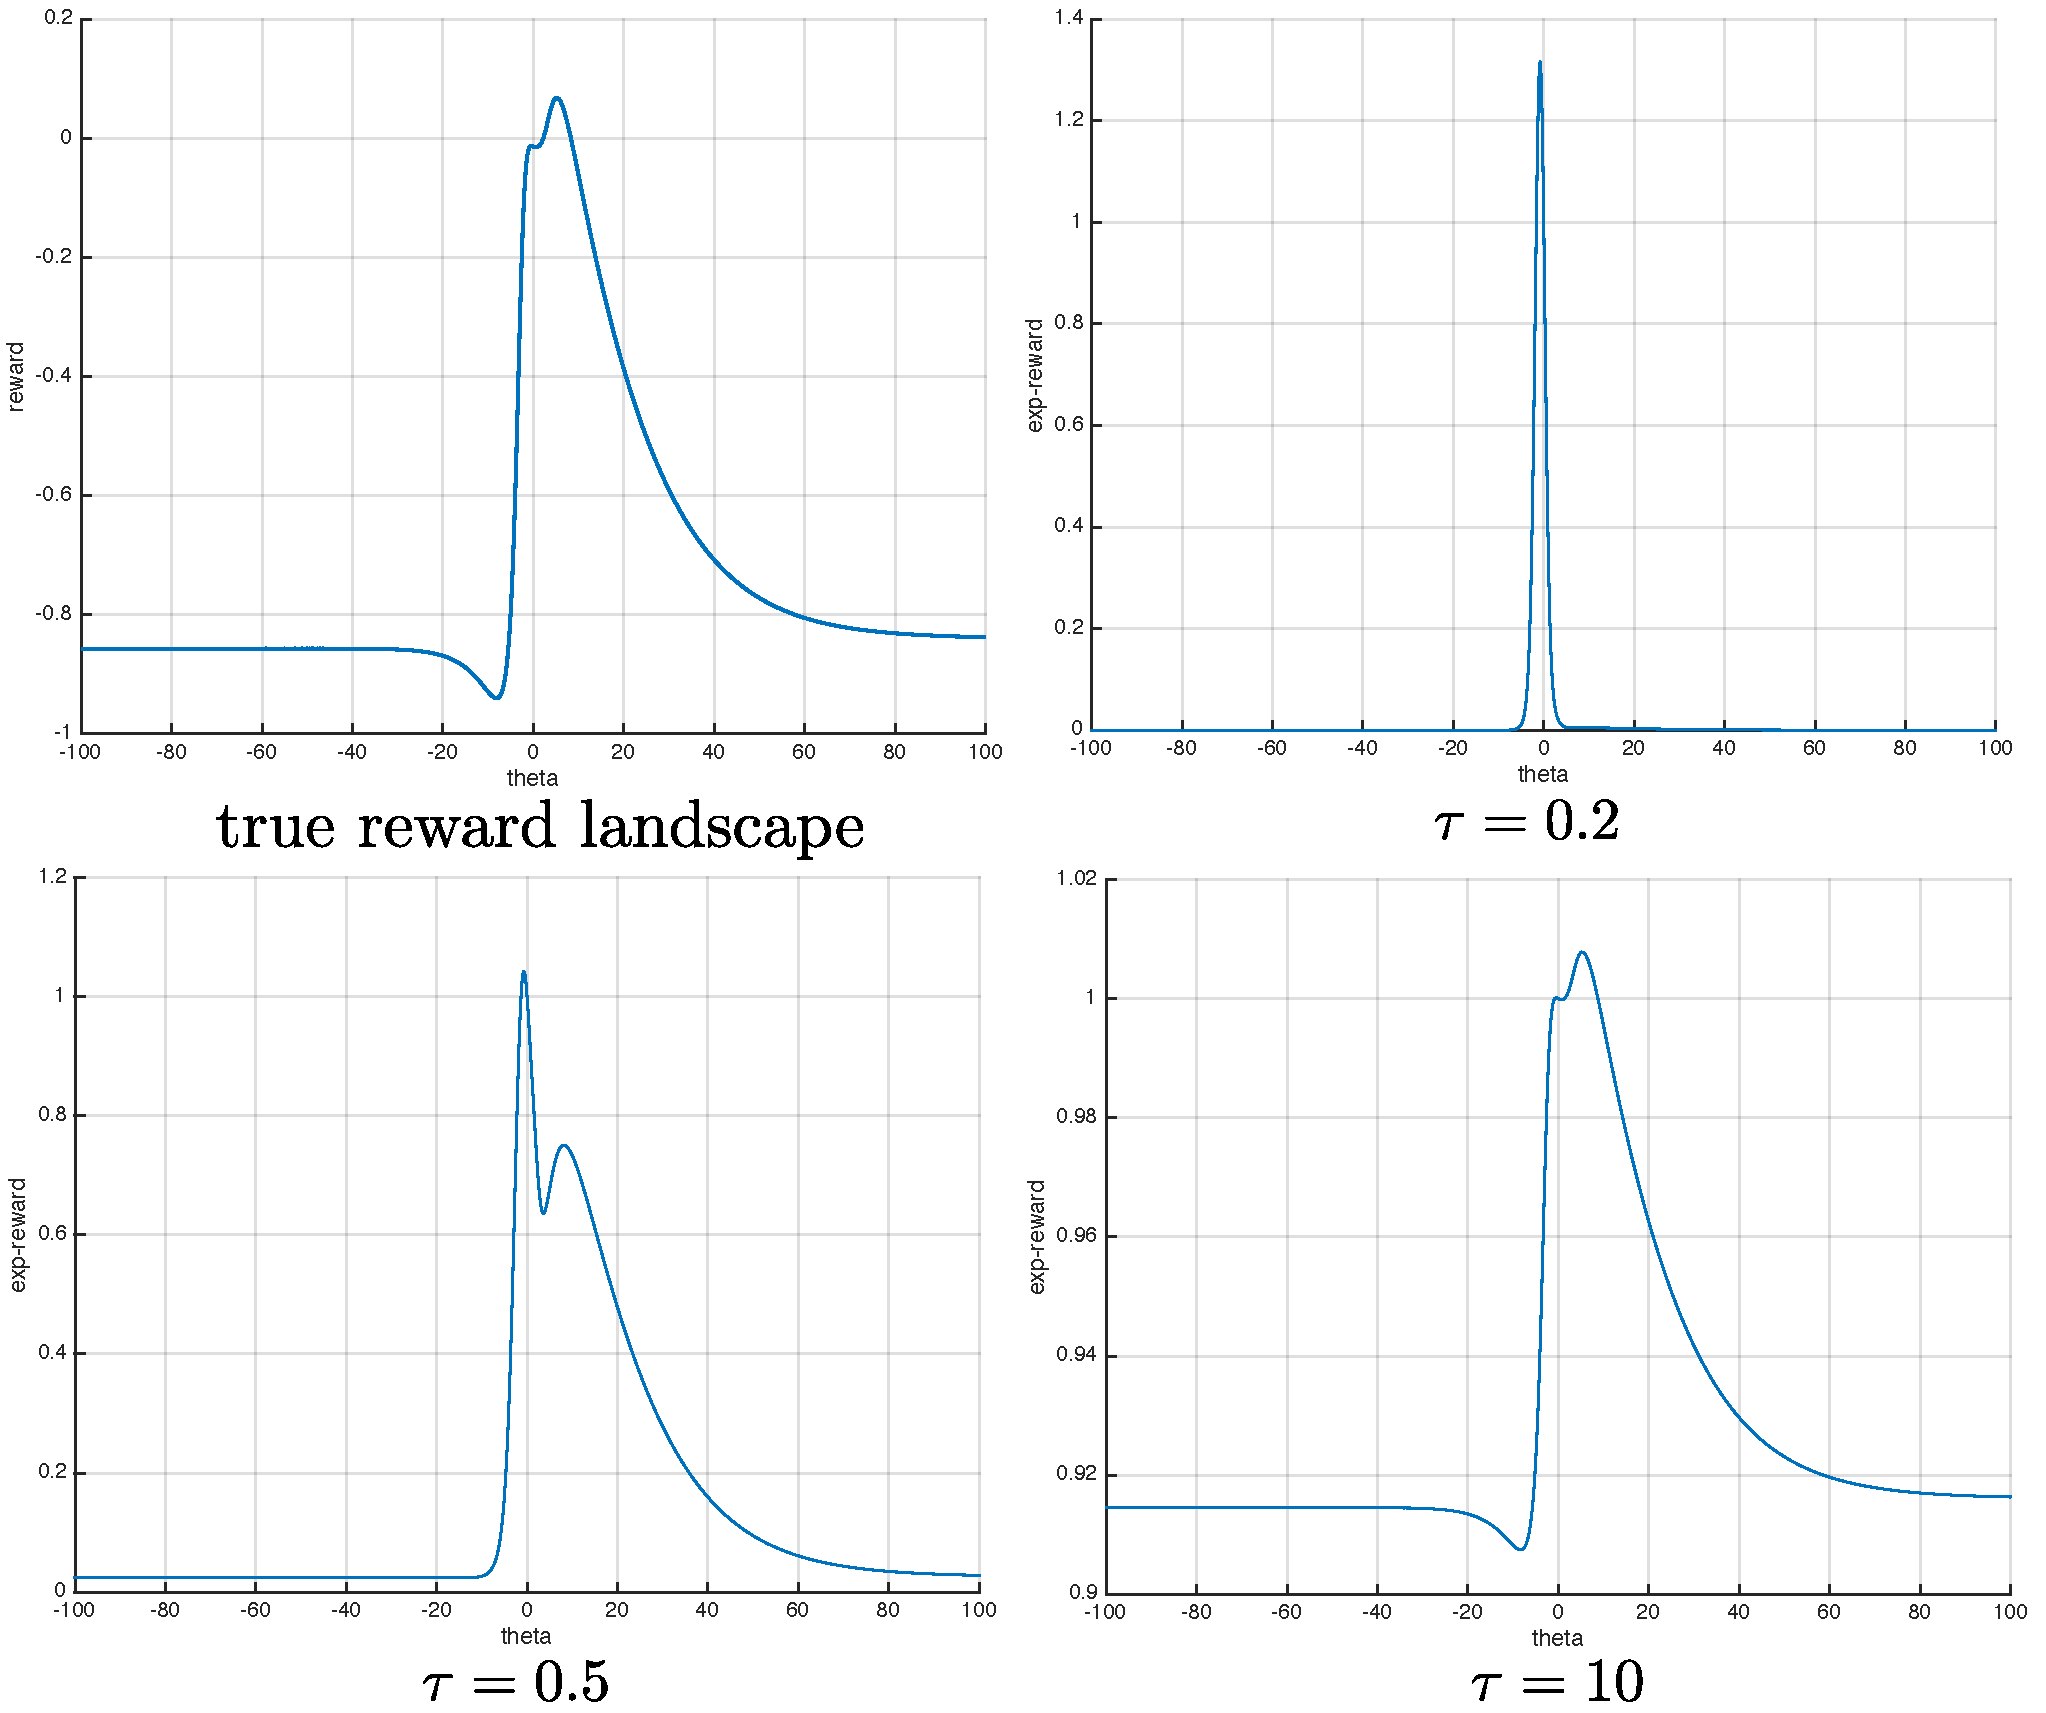
\includegraphics[width=0.38\linewidth]{par_reward.pdf}}
%\parpic[r]{\fbox{\rule{2.35in}{0in}\rule{0in}{2.0in}}}
\vspace{-0.2cm}

{\bf Reviewer 2: }
%
Thanks for the helpful comments.
It is indeed interesting to investigate the effect on problem structure as 
$\tau$ and $\tau^\prime$ vary.
Figure~\ref{fig:exp_reward_over_theta} shows a preliminary investigation
using the same setting as in Sec 4.1.1 with $\theta \in \mathbb{R}$ as a scalar.
When $\tau$ is small $(\tau =0.2)$,
the exp-reward landscape provides good guidance for maximizing the true reward.
As $\tau$ increases, local maxima appear as the exp-reward approaches the
true reward landscape.
The impact of varying $\tau^\prime$ is also worth exploring;
we would be happy to include
performance sensitivity to $\tau$ and $\tau^\prime$.

{\bf Reviewer 3: }
%
First, to clarify the technical questions:

Regarding $\pi(\rho)$:
$\text{Pr}(\rho) = \pi(\rho) p(\rho) \triangleq
\prod_{t=1}^{T-1}{ \pi(a_t | s_t) p(s_{s+1} | s_t, a_t)}$, 
where $p$ is the transition probability depends on $f$. 
As in Line 47, we assume $p(s_{s+1} | s_t, a_t) = 1$ for clarity, 
hence $\sum_{\rho}{\pi(\rho)} = \sum_{\rho}{\text{Pr}(\rho)} = 1$.
As in [11] this sacrifices no generality.
The stochastic case can be detailed in the supplement,
but this has no impact on the method.

%{\bf [I think you misunderstand the reviewer's question.]}
%Regarding $\pi_{\tau}^{*}$:
%Consider Eq. (2) without the $\Pi$ constraint and take the stochastic
%transition probability into account;
%we have 
%$\max_{\pi \in \{ \pi | \sum_{\rho}{\pi(\rho)p(\rho) = 1} \}}
%{\sum_{\rho}{\pi(\rho)p(\rho)[ r(\rho) - \tau \log{\pi(\rho)}]}}$.
%The KKT condition is 
%$p(\rho) [ r(\rho) - \tau \log{\pi(\rho)  - 1 + \lambda]} = 0$, $\forall \rho$.
%Since we take expectation on every actual trajectory $\rho$, we have 
%$p(\rho) > 0$.
%Thus the KKT condition does not involve $p(\rho)$, and the solution
%$\pi_{\tau}^{*}$ will not change.

Regarding $\pi_{\tau}^{*}$:
It is straightforward to verify that 
the solution to Eq.(2) without the constraint $\Pi$
is given by $\pi_{\tau}^{*}$ as shown in Line~63.
However, the algorithm never needs to compute the denominator in
$\pi_{\tau}^{*}$.
%To further optimize over $\pi_\theta$ in $\Pi$ or solve Eq.(5),
%one does NOT need the value of $\pi_{\tau}^{*}$. 
Instead, the algorithm uses importance sampling to sample trajectories from
$\pi_{\tau}^{*}$ to optimize $\pi_\theta$.
Similar ideas are also applied to $\bar{\pi}_\tau^*$ in Eq.(5). 

Mode seeking vs.\ mode covering:
The effects of minimizing different orientations of KL divergence are
well known; see Sec 21.2.2 in [7, Murphy 2012].
In particular, minimizing $\text{KL}(\pi_{\theta}\|q)$
usually underestimates the support of $q$,
since the objective is infinite if $q = 0$ and $\pi_{\theta} > 0$.
Thus, $\pi_\theta$ is driven to $0$ wherever $q=0$.
The problem is that when $q$ changes, $\pi_\theta$ can have zero mass
on trajectories that have non-zero probability under the new $q$,
hence $\pi_\theta$ will never capture this part of $q$,
leading to mode collapse.
By contrast, minimizing $\text{KL}(q\|\pi_{\theta})$ 
is zero-avoiding in $\pi_{\theta}$,
since if $q > 0$ we must ensure $\pi_{\theta} > 0$.
Note that by Eq.(7):
(a) the $q$ in our method is nonzero everywhere,
(b) we further add entropy in Eq.(6) to avoid $q$ prematurely converging
to a deterministic policy, 
(c) $\text{KL}(q\|\pi_{\theta})$ is zero-avoiding for minimization over
$\pi_{\theta}$.
These ensure that the proposed method does not exhibit the same mode-seeking 
behavior as MD.

Effect of changing $K$:
We did conduct some experiments for a larger $K = 20$, and found that it does
reduce the number of iterations needed to reach optima,
but does not change the optimal values achieved.
More experiments are ongoing.

\if0
\newpage

\section{Old}

R1: 
1. We thank the reviewer for the referred papers. [Liu et al., UAI 2015] is not directly relevant to our paper. Although both are inspired by the MD framework,
our setting/result is very different with that in [Liu et al., UAI 2015]. Liu et al. consider the value evaluation of fixed policy, while this work focuses on trajectory based policy optimization (controlling setting). On the other hand, our paper indeed shares similarities with [Thomas et al., NIPS 2013], but only in a high level that both optimizing the policy in the MD framework and then perform a projection step. These two works still differ in many ways, including the motivation, the results, and the technique part. The focus of our paper is to investigate the exploration behavior of the method while Thomas et al. focus on learning safe policies. We proved some nice theoretical properties of our method in our paper (even in the non-convex setting, see the next comment for details), while the method of Thomas et al. is proposed heuristically and it is not clear if these good properties would hold. Lastly on the technical side, Thomas et al. follow the standard MD framework, while we propose to use the reverse direction of KL divergence. We will cite these papers and discuss their differences in our paper.

2. In fact, the analyses of the proposed REPMD algorithm in the non-convex settings is one of the most important contributions of this paper. Many good properties about the MD framework only hold under the convexity assumption, which limits the application of the standard MD methods. However, all the propositions and theorems in our paper does NOT require the convexity assumption, but only that the optimization problems in Eq. (6) can be solved: (1) Solving $\bar{\pi}^*_{\tau, \tau'}$ is a non-convex problem, but we showed that it actually has a analytical solution; (2) Solving the projection step, $\pi_\theta$, is still difficult for a general neural network parametrization, but it is solvable in some particular non-convex cases. Consider the widely used parameterized softmax policies $\pi_{\theta} \triangleq \frac{\exp\left\{\Phi^\top\theta\right\}}{{\mathbf{1}^\top \exp\left\{\Phi^\top\theta\right\} }}$, where $\Phi\in \mathbb{R}^{A\times K}$ is the feature matrix, $A$ is the number of actions, $K$ is the dimension of features, and $\theta$ is the policy parameter. Note that the policy space is non-convex and $K\ll A$ as in Sec 4.1.1. Standard MD cannot exactly solve this projection step because $\text{KL}(\pi_{\theta} \| q)$ is non-convex in $\theta$. On the other hand, our paper proposes to use the reversed entropy $\text{KL}(q \| \pi_{\theta})$, which is actually convex for $\theta$ (note that $\frac{d^2 \text{KL}(q \| \pi_{\theta})}{d \theta^2} = \Phi^\top (\Delta(\pi_\theta) - \pi_\theta \pi_\theta^\top) \Phi \succeq 0$). It is also worth noting this is the 1-layer NN case. For more general NN architectures, further understanding of the behavior of NN is needed to make progress here. We will add this claim and the proof to the paper.

\if0
An important contribution is: there are non-convex problems where our method has advantage over MD. Consider widely used parameterized softmax policies $\pi_{\theta} \triangleq \frac{\exp\left\{\Phi^\top\theta\right\}}{{\mathbf{1}^\top \exp\left\{\Phi^\top\theta\right\} }}$, where $\Phi\in \mathbb{R}^{A\times K}$ is the feature matrix, $A$ is the number of actions, $K$ is the dimension of features, and $\theta$ is the policy parameter. Note that the policy space is non-convex and $K\ll A$ as in Sec 4.1.1. Standard MD cannot solve its projection exactly because $\text{KL}(\pi_{\theta} \| q)$ is non-convex for $\theta$. On the other hand, our paper proposes to use the reversed entropy $\text{KL}(q \| \pi_{\theta})$ so that,  our method can solve its projection, because $\text{KL}(q \| \pi_{\theta})$ is convex for $\theta$ $(\frac{d^2 \text{KL}(q \| \pi_{\theta})}{d \theta^2} = \Phi^\top (\Delta(\pi_\theta) - \pi_\theta \pi_\theta^\top) \Phi \succeq 0)$. In a word, our method guarantees monotonic performance improvement (Thm 1), while the corresponding property of original MD (Prop 3) cannot hold.
\fi 


3) [Thomas et al., NIPS 2013] indeed has interesting simulated and robotic experiments, but it is debatable that it is a better setting. a) Comparing with real world, it is still oversimplified. On the other hand, benchmark tasks help align different research results in the community. Using relatively complicated yet non-open-source settings may bring unnecessarily difficulty in reproducibility of the results and understanding the fundamental properties of different methods. b) Existing RL methods are not  yet powerful enough even for difficult simulation problems. For example, to our best knowledge, no purely policy based method can solve all the OpenAI Algorithmic tasks. Also, currently no standard RL method can solve difficult video games like Super Mario Bro and Montezuma's Revenge without human demonstration. Since ``the issue of sample complexity'' is very crucial in real world, we need better understanding of principled exploration. Before conquering difficult simulation problems with low sample complexity, it is hard to argue that current technology has efficiently solved the real world problems. c) The experiments are to verify that our method is a more efficient exploration than existing methods in principle. For our method to outperform the current state-of-the-art results on some complicated tasks, it will probably also need the help of other practical tricks and models, but this is beyond the scope of this paper, which is trying to understand the exploration behavior of different methods in principle.

\piccaption[]{reward and exp-reward over $\theta$.\label{fig:exp_reward_over_theta}}
\parpic[r]{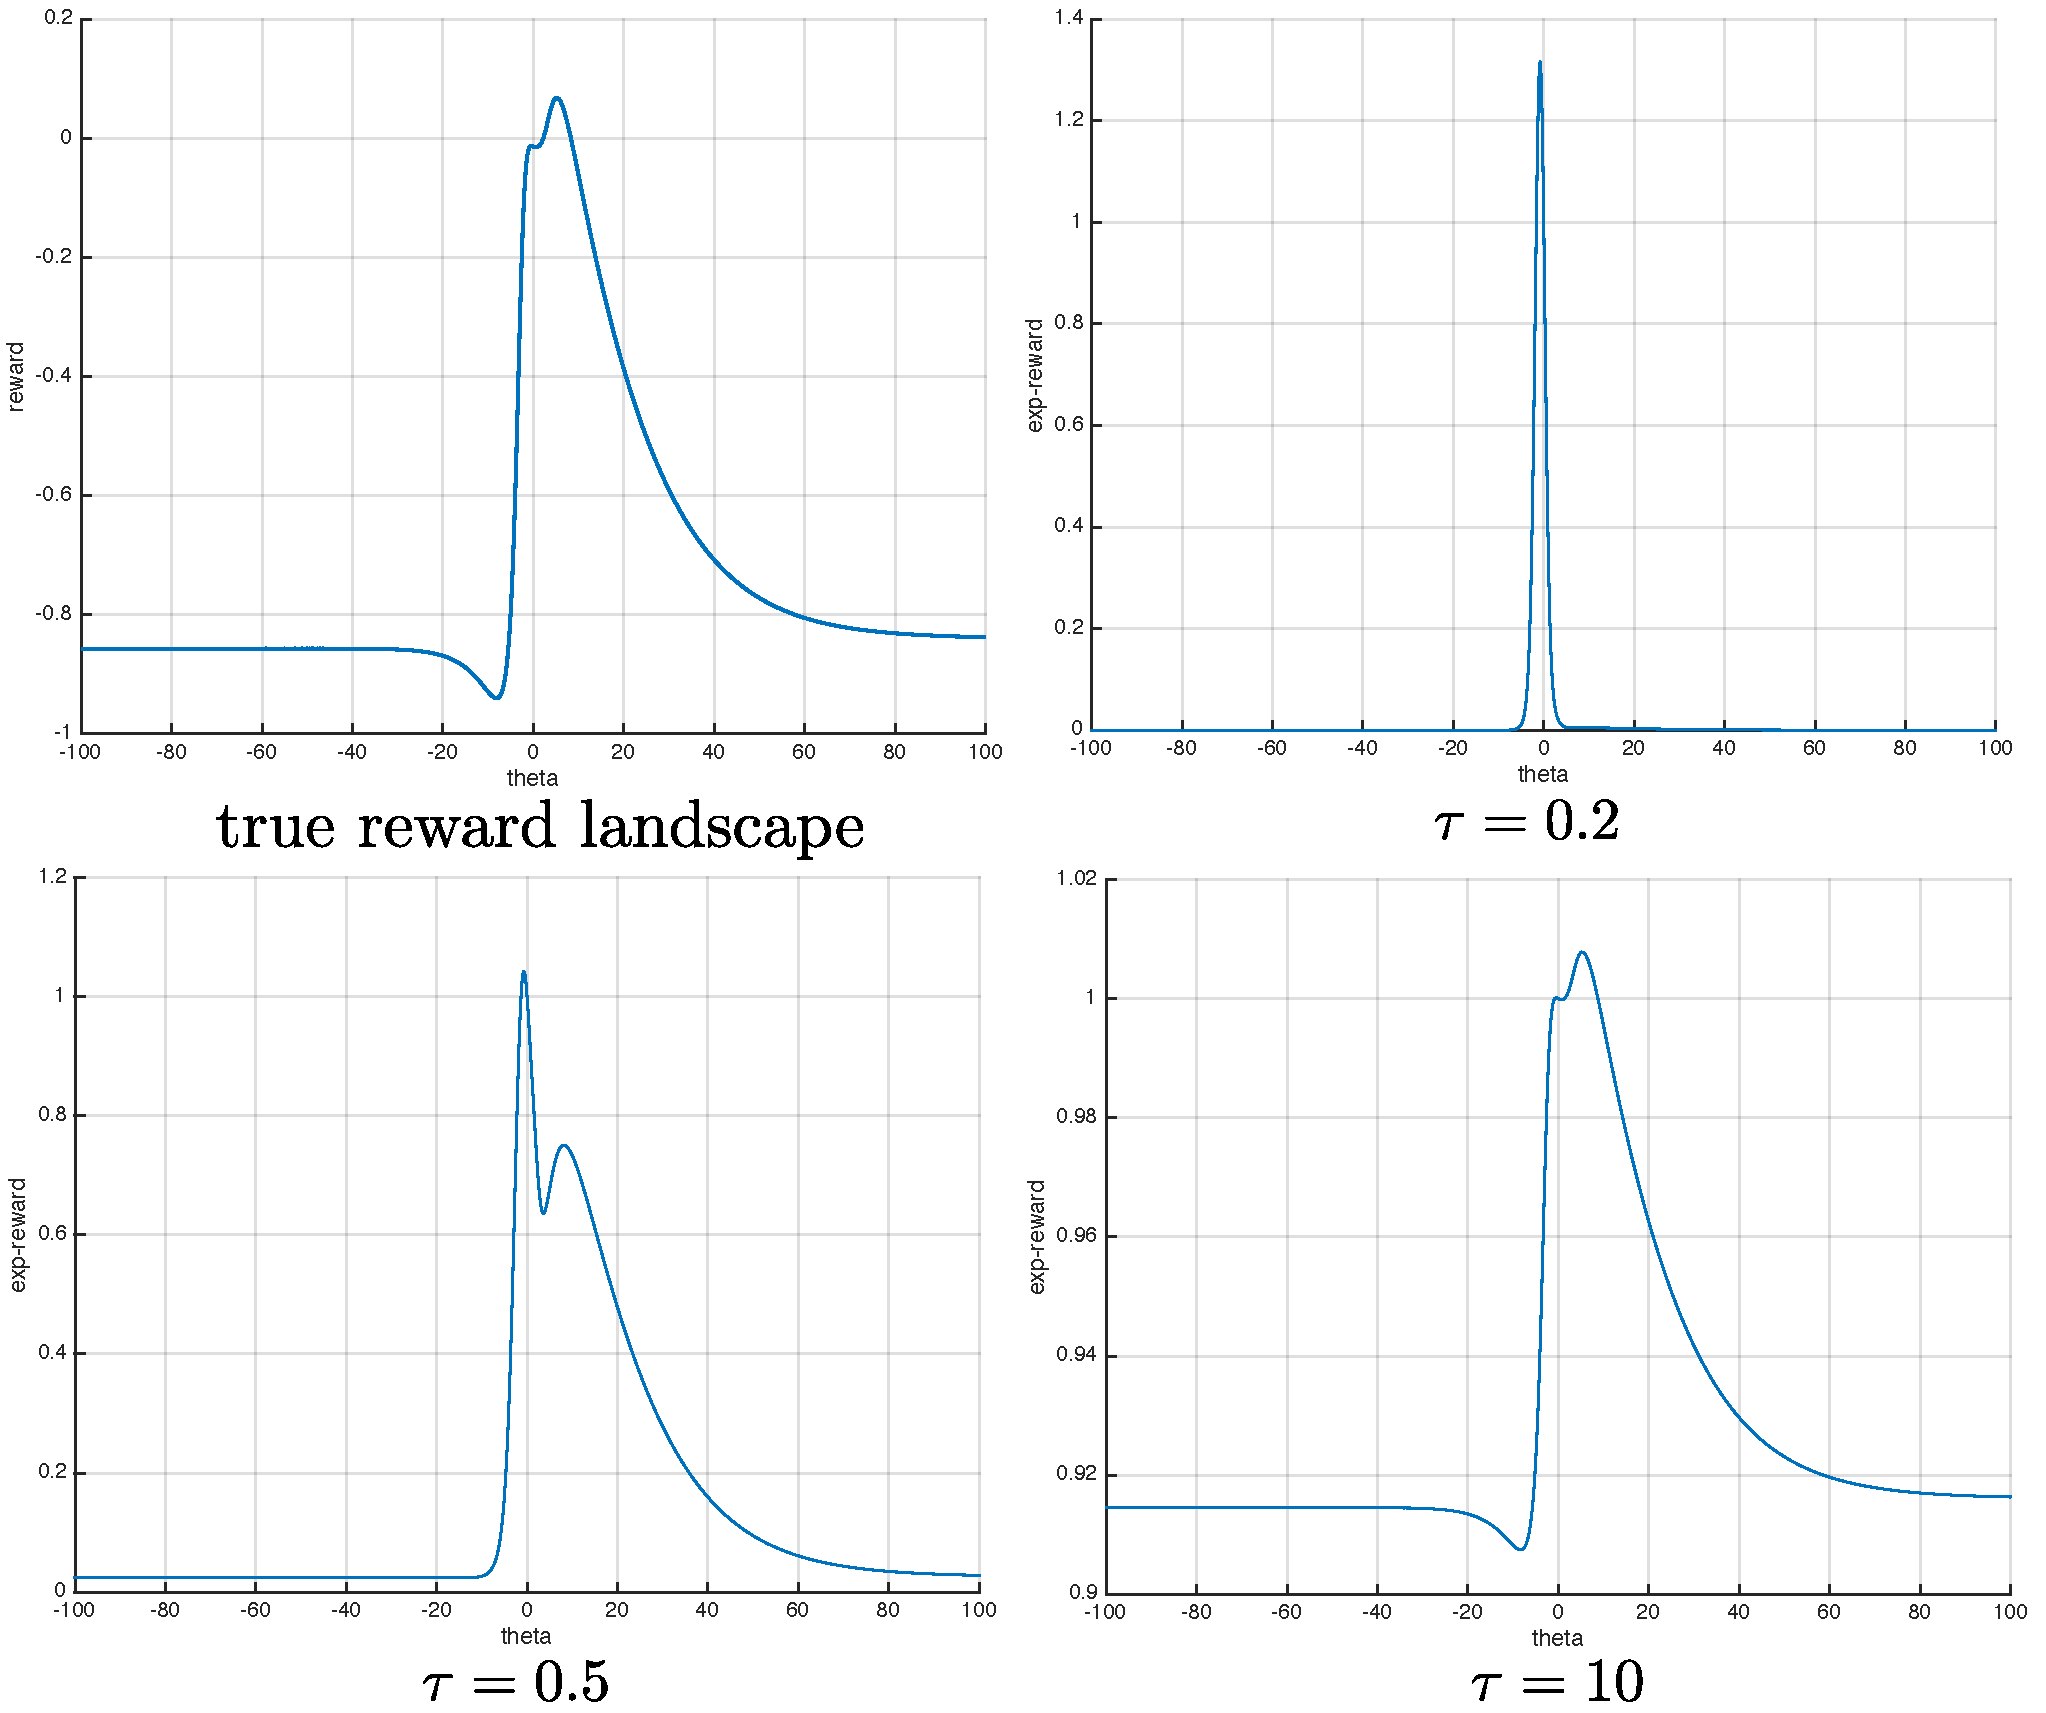
\includegraphics[width=0.38\linewidth]{par_reward.pdf}}

R2: Thank you for helpful comments. It is indeed interesting to investigate the 
change of problem structure as the parameters $\tau$ and $\tau^\prime$ vary. 
We did some preliminary investigation, as shown in Figure \ref{fig:exp_reward_over_theta}, using the same setting as in Sec 4.1.1 with $\theta \in \mathbb{R}$ as a scalar. When $\tau$ is small $(\tau =0.2)$, the exp-reward landscape is a good guidance for maximizing the true reward, as it remedies the problem that directly maximizing the true reward will converges to negative infinity when $\theta$ is initialized on the left hand side. As $\tau$ increases, local maxima appear while it is getting closer to the true reward landscape. For relatively large $\tau = 10$, exp-reward looks nearly identical with the true reward landscape. The impact of varying $\tau^\prime$ is also worth exploring. Actually in our reported experiments, we gradually increase $\tau$ and decrease $\tau^\prime$ and we find this works well. We will report the detail. Further investigation will be made to figure out the detailed impact of $\tau$ and $\tau^\prime$ and to find a principled rule or method to adjusting these two parameters. We will report the numerical results for the sensitivity of performance over the parameters $\tau$ and $\tau^\prime$.

R3:
The results are technically sound. To clarify your concerns:

 1) $\pi(\rho)$: $\text{Pr}(\rho) = \pi(\rho) p(\rho) \triangleq \prod_{t=1}^{T-1}{ \pi(a_t | s_t) p(s_{s+1} | s_t, a_t)}$, where $p$ is the transition probability depends on $f$. As in Line 47, we assume deterministic transition for simplicity, i.e., $p(s_{s+1} | s_t, a_t) = 1$. So $\sum_{\rho}{\pi(\rho)} = \sum_{\rho}{\text{Pr}(\rho)} = 1$. Note that by assuming deterministic transition function we lose no generality. The same idea is also used in [11]. We  will add generalization to stochastic transition in supplementary for completeness, which has no impact on the method.

2) [I think you misunderstand the reviewer's question.] $\pi_{\tau}^{*}$: Consider Eq. (2) without $\Pi$ constraint and take stochastic transition probability into account, we have $\max_{\pi \in \{ \pi | \sum_{\rho}{\pi(\rho)p(\rho) = 1} \}}{\sum_{\rho}{\pi(\rho)p(\rho)[ r(\rho) - \tau \log{\pi(\rho)}]}}$. The KKT condition is $p(\rho) [ r(\rho) - \tau \log{\pi(\rho)  - 1 + \lambda]} = 0$, $\forall \rho$. Since we take expectation on every actual trajectory $\rho$, we have $p(\rho) > 0$. Thus the KKT condition does not involve $p(\rho)$, and the solution $\pi_{\tau}^{*}$ will not change.

$\pi_{\tau}^{*}$ as the optimal solution for Equation (2),  its analytical formula can be computed as shown in Line 63. However, the algorithm does NOT need to evaluate its value. To further optimize over $\pi_\theta$ in $\Pi$ or solve Eq. (5), one does NOT need the value of $\pi_{\tau}^{*}$. Instead, the algorithm uses importance sampling to sample trajectories from $\pi_{\tau}^{*}$ to optimize $\pi_\theta$. Similar ideas are also applied to $\bar{\pi}_\tau^*$ in Eq. (5). 

3) mode: It is well known that KL divergence is mode-seeking, while the reversed direction of it is mean-seeking. See for example Sec 21.2.2 in [7, Murphy 2012]. In particular, minimizing $\text{KL}(\pi_{\theta} || q)$ usually underestimates the support of $q$, since KL is infinite if $q = 0$ and $\pi_{\theta} > 0$. This KL optimization is zero-forcing $\pi_{\theta} $. When $q$ changes, some part of $\pi_{\theta} = 0$ by the previous KL optimization, $\pi_{\theta}$ can never collect this part trajectories ($\pi_{\theta} = 0$), thus it cannot learn to modify this part to be close to the new $q$. Repeatedly happening things like this will lead $\pi_{\theta}$ collapse to some modes. While $\text{KL}(q || \pi_{\theta})$ is zero-avoiding $\pi_{\theta}$, since if $q > 0$ we must ensure $\pi_{\theta} > 0$ for minimization [7]. Note Eq. (7) in the paper, a) $q$ in our method is nonzero everywhere, b) we add entropy in Eq. (6) to avoid $q$ early converge to deterministic policies, c) $\text{KL}(q || \pi_{\theta})$ is zero-avoiding for minimization over $\pi_{\theta}$. These ensures our method is not mode-seeking as MD.

4) We did experiments for larger $K = $, and we find that... 
\fi

\textcolor{red}{Dale's comment}

\textcolor{red}{
\sout{R1: 1) quick thanks, 
But ref1 not the same setting, we consider policy optimization; ref2, we have proved properties which ref2 does not have/they can't prove/they do not consider. So the contribution of the paper has been ignored.}}

\textcolor{red}{\sout{2) more direct: there are non-convex problems that our proposed method can solve, while mirror descent cannot. Our contribution has been misunderstood.}}

\textcolor{red}{\sout{3) ref2 has interesting experimental setting, but it can not be concluded that it is better than ours. For experiments, we need to consider the reproducibility and simplicity. We chose benchmark publicly available rather than problems that complicated to reproduce, which is helpful for understanding of basic exploration problem.}}

\textcolor{red}{\sout{R2: helpful comments and corrections.}}

\textcolor{red}{
\sout{R3:
1) technical issue, need more response: pointing politely that the reviewer misunderstood/did not carefully read the paper. make each issue clarified.
}}

\textcolor{red}{
\sout{2) mode-seeking: good, too long
}}

\textcolor{red}{
\sout{3) weak: run some experiments, show the results and conclusions
}}

\end{document}
